% !TEX TS-program = pdflatex
% !TEX encoding = UTF-8 Unicode

% This is a simple template for a LaTeX document using the "article" class.
% See "book", "report", "letter" for other types of document.

\documentclass[11pt]{article} % use larger type; default would be 10pt

\usepackage[utf8]{inputenc} % set input encoding (not needed with XeLaTeX)

%%% Examples of Article customizations
% These packages are optional, depending whether you want the features they provide.
% See the LaTeX Companion or other references for full information.

%%% PAGE DIMENSIONS
\usepackage{geometry} % to change the page dimensions
\geometry{a4paper} % or letterpaper (US) or a5paper or....
% \geometry{margin=2in} % for example, change the margins to 2 inches all round
% \geometry{landscape} % set up the page for landscape
%   read geometry.pdf for detailed page layout information

\usepackage{graphicx} % support the \includegraphics command and options

% \usepackage[parfill]{parskip} % Activate to begin paragraphs with an empty line rather than an indent

%%% PACKAGES
\usepackage{booktabs} % for much better looking tables
\usepackage{array} % for better arrays (eg matrices) in maths
\usepackage{paralist} % very flexible & customisable lists (eg. enumerate/itemize, etc.)
\usepackage{verbatim} % adds environment for commenting out blocks of text & for better verbatim
\usepackage{subfig} % make it possible to include more than one captioned figure/table in a single float
\usepackage{amsmath}
\usepackage{mathtools}
\usepackage[thinc]{esdiff}
% These packages are all incorporated in the memoir class to one degree or another...

%%% HEADERS & FOOTERS
\usepackage{fancyhdr} % This should be set AFTER setting up the page geometry
\pagestyle{fancy} % options: empty , plain , fancy
\renewcommand{\headrulewidth}{0pt} % customise the layout...
\lhead{}\chead{}\rhead{}
\lfoot{}\cfoot{\thepage}\rfoot{}

%%% SECTION TITLE APPEARANCE
\usepackage{sectsty}
\allsectionsfont{\sffamily\mdseries\upshape} % (See the fntguide.pdf for font help)
% (This matches ConTeXt defaults)

%%% ToC (table of contents) APPEARANCE
\usepackage[nottoc,notlof,notlot]{tocbibind} % Put the bibliography in the ToC
\usepackage[titles,subfigure]{tocloft} % Alter the style of the Table of Contents
\renewcommand{\cftsecfont}{\rmfamily\mdseries\upshape}
\renewcommand{\cftsecpagefont}{\rmfamily\mdseries\upshape} % No bold!

%%% END Article customizations

%%% The "real" document content comes below...

\title{BIOS 767 HW1}
\author{Mingwei Fei}
%\date{} % Activate to display a given date or no date (if empty),
         % otherwise the current date is printed 

\begin{document}
\maketitle

\section{Problem 1 - Computing moments}
Consider the following model for subject i in group h at time j:
 
\begin{align*}
	Y_{hij} &= \mu + \alpha_h + \beta_j + \gamma_{hj} + b_{hi} + \epsilon_{hij}
\end{align*}

where $b_{hi} \sim N(0, \sigma^2_b)$ and $\epsilon_{hij} \sim N(0, \sigma^2_e)$, for $h=1,..H, i=1,..n_h,$ and $j=1,.. J$. Assume that random variables that do not share a common value of h or i are independent. 

\begin{itemize}
\item[(a)] Compute $E[Y_{hij}]$.
	
	\begin{align*}
		Y_{hij} &= \mu + \alpha_h + \beta_j + \gamma_{hj} + b_{hi} + \epsilon_{hij} \\
		E[Y_{hij}] &= \mu + \alpha_h + \beta_j + \gamma_{hj} + E[b_{hi}] + E[\epsilon_{hij}] \\
		 E[b_{hi}] &= 0, \qquad E[\epsilon_{hij}] = 0, \qquad \text{as} \quad b_{hi} \sim N(0, \sigma^2_b), \epsilon_{hij} \sim N(0, \sigma^2_e) \\
		E[Y_{hij}] &= \mu + \alpha_h + \beta_j + \gamma_{hj} 
	\end{align*}

\item[(b)] Don't assume $b_{hi}$ and $\epsilon_{hij}$ are independent. Derive an expression for $Var[Y_{hij}]$ that it as simplified as possible.

If $b_{hi}$ and $\epsilon_{hij}$ are not independent,
\begin{align*}
	Var[b_{hi} + \epsilon_{hij}] &= Var[b_{hi}] + Var[\epsilon_{hij}] +2 Cov[b_{hi}, \epsilon_{hij}] \\
	Y_{hij} &= \mu + \alpha_h + \beta_j + \gamma_{hj} + b_{hi} + \epsilon_{hij} \\
	Var[Y_{hij}] &= Var[b_{hi} + \epsilon_{hij}] \\
	Var[b_{hi}] &= \sigma^2_b, \qquad Var[\epsilon_{hij}] = \sigma^2_e, \qquad \text{as} \quad b_{hi} \sim N(0, \sigma^2_b), \epsilon_{hij} \sim N(0, \sigma^2_e) \\
	Var[Y_{hij}] &= \sigma^2_b + \sigma^2_e + 2 Cov[b_{hi}, \epsilon_{hij}]
\end{align*}

\item[(c)] assume $b_{hi}$ and $\epsilon_{hij}$ are independent. Derive an expression for $Var[Y_{hij}]$. 

If $b_{hi}$ and $\epsilon_{hij}$ are independent,
\begin{align*}
	Cov[b_{hi}, \epsilon_{hij}] &= 0\\
	Var[Y_{hij}] &= \sigma^2_b + \sigma^2_e
\end{align*}

\end{itemize}

\section{Problem 2 - Correlation in Data}
Consider the general linear regression model:

\begin{align*}
	Y_{n \times 1} &= X_{n \times p} \beta + \epsilon_{n \times 1}
\end{align*}

where $\epsilon$ is normal, and $\theta$ is unknown.

\begin{itemize}
	\item [(a)] Show the the ordinary least squares (OLS) estimator $\hat{\beta}^{OLS}$ is unbiased.
	We need to show $E(\hat{\beta}^{OLS}) = \beta$
\begin{align*}
	\hat{\beta}^{OLS} &=  (X^T X)^{-1}X^T Y \\
	E(\hat{\beta}^{OLS}) &= (X^T X)^{-1}X^T E(Y) =  (X^T X)^{-1}X^T X \beta = \beta
\end{align*}	
	
	\item[(b)] Derive the variance of $\hat{\beta}^{OLS}$ 
	
\begin{align*}
	Var(\hat{\beta}^{OLS}) &= Var((X^T X)^{-1}X^T Y )= (X^T X)^{-1}X^T Var(Y) [(X^T X)^{-1}X^T ]^T \\
	Var(Y) &= \Sigma \\
	Var(\hat{\beta}^{OLS})  & =  (X^T X)^{-1}X^T \Sigma X [(X^T X)^{-1}] 
\end{align*}		
	if X is non-singular, we can further simplify 
\begin{align*}	
	Var(\hat{\beta}^{OLS})	&= X^{-1} (X^T)^{-1} X^T \Sigma X X^{-1} (X^T)^{-1} \\
	&= X^{-1} \Sigma (X^T)^{-1} = [X^T \Sigma^{-1} X]^{-1}
\end{align*}		
	
	\item[(c)] Derive an expression for the variance of $\hat{\beta}^{OLS}$ (simplified as much as possible).
	
	\begin{align*}
	\Sigma &= \sigma^2 I_{n \times n} \\
	Var(\hat{\beta}^{OLS}) &= [X^T \Sigma^{-1} X]^{-1} = \sigma^2 (X^T X)^{-1}
\end{align*}

\item[(d)] Now, assume n = 10, p = 1, and let X be a vector of ones (e.g., an intercept only model). $\rho in (0,1)$, plot the true standard deviation of $\hat{\beta}^{OLS}$ as a function of $\rho$.

\begin{align*}
	\Sigma &= \sigma^2 I_{n \times n} = \begin{pmatrix}
	1 & \rho &.. & \rho \\
	\rho & 1 &.. & \rho\\
	.. &.. & ..& \\
	\rho & \rho &. .& 1  
	\end{pmatrix}
\end{align*}

The plot of SD as a function of $\rho$ as below:
\begin{figure}[h]
	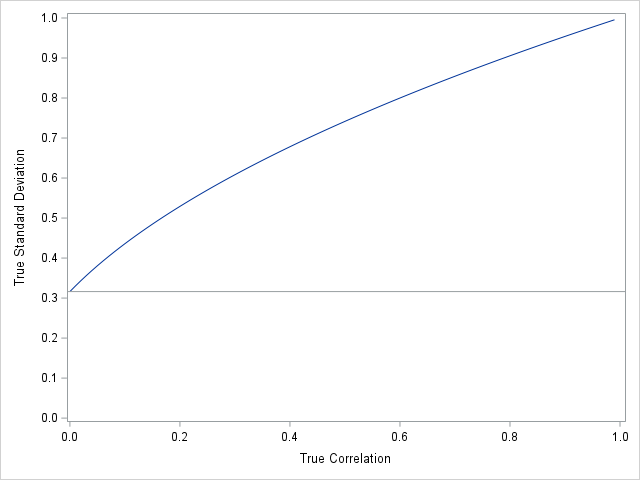
\includegraphics[width=15cm]{2d.png}
\end{figure}

\item[(e)] From the previous example, as $\rho \rightarrow 1 $, you should observe that the true SD for $\hat{\beta}_{OLS} \rightarrow 1$. Concisely state why this is the case using one or two complete sentences.

From the SD formula, we calculate 
\begin{align*}
	\Sigma &= \begin{pmatrix}
		1 & \rho &.. & \rho \\
		\rho & 1 &.. & \rho\\
		.. &.. & ..& \\
		\rho & \rho ..&. & 1 
	\end{pmatrix} = \begin{pmatrix}
	1 & 1 &.. & 1 \\
	1 & 1 &.. & 1 \\
	.. &.. & ..& \\
	1 & 1 &. .& 1 
\end{pmatrix} , \qquad \rho \rightarrow 1\\
X &= (1,...1)^T,  X^T X = 10 \\
	Var(\hat{\beta}^{OLS}) & = (X^T X)^{-1}X^T \Sigma X [(X^T X)^{-1}] \\
	&= 10^{-1} (1,...1) \begin{pmatrix}
		1 & 1 &.. & 1 \\
		1 & 1 &.. & 1 \\
		.. &.. & ..& \\
		1 & 1 &. .& 1 
	\end{pmatrix} _{10 \times 10} (1,...1)^T 10^{-1} \\
&= 10^{-1} (10,...10) (1,...1)^T 10^{-1}  = 1\\
\end{align*}

When correlation coefficient is 1, we have the covariance is the same as variance, which shows that there is only one estimate, ie. overall mean. So the variance of the estimate is the variance of response variable or error term, which is 1.

\item[(f)] Hypothesis test of $\beta$. They do so using the OLS estimator but erroneously assume independent covariance matrix. when in fact the correlation between observations$\rho = \frac{1}{n-1}$. Note that, in this case is equal to the sample mean. What is the actual type I error rate for this test? What can you say about the impact of ignoring even small positive correlation in ananalysis when the sample size is large?

Assume we have the $\hat{\beta} $ based on the correlated covariance matrix. The incorrect variance is $\frac{1}{n}$
The p-value for two sided rejection region (type I error) is 
\begin{align*}
	\hat{\beta}  &= (X^T X)^{-1}X^T \Sigma X [(X^T X)^{-1}] \\
	p(x > \hat{\beta} | \beta = 0) &= p(x <- \hat{\beta} |  \beta = 0) \\
	Z &= \frac{ \hat{\beta} - 0}{\sqrt{1/n}} \\
	p &= 2 p(x <- \hat{\beta} | \beta = 0) = 2 CDF(-Z)
\end{align*}

So we will have inflated type I error if using the independent covariance matrix. The actual type I error rate is $ 0.16618$ from the simulated code.

When sample size is large, the impact of ignoring the small positive correlation will become signficant as the true standard deviation is much larger than sd assuming independence $\sqrt{1/n}$. In turn, it would cause more inflated type I error.
 
\end{itemize}

\section{Problem 3- Naive approach to handle correlation in Data}

Consider the subject-specific linear regression model:
\begin{align*}
	Y_{hij}  &= \beta_{h0} + t_{hij} \beta_{h1} + \epsilon_{hij} \\
	\hat{\beta}_{hi} &= (\hat{\beta}_{hi,0}, \hat{\beta}_{hi,1})^T = (X_{hi}' X_{hi})^{-1} X_{hi}' Y_{hi}
\end{align*}
The analyst plans to test the hypotheses 
\begin{align*}
	H_0:   &= \beta_{11} = \beta_{21} vs. H_1: \beta_{11} \neq \beta_{21}
\end{align*}
using a two-sample t-test using the values $\hat{\beta}_{hi,1}: h= 1,2 ; i= 1,..n $ 

\begin{itemize}[]
	
	\item[(a)] Compute $E[\hat{\beta}_{hi} ], Var[\hat{\beta}_{hi} ], Var[\hat{\beta}_{hi,1} ]$. 
\begin{align*}
		\hat{\beta}_{hi} &= (X_{hi}' X_{hi})^{-1} X_{hi}' Y_{hi} \\
	E(\hat{\beta}_{hi}) &= (X_{hi}' X_{hi})^{-1} X_{hi}' E[Y_{hi}] \\
	& =  (X_{hi}' X_{hi})^{-1} X_{hi}' X_{hi} \beta_{hi} =\beta_{hi} 
\end{align*}	

the variance 
\begin{align*}
	Var(\hat{\beta}_{hi}) &= Var \Big((X_{hi}' X_{hi})^{-1} X_{hi}' Y_{hi} \Big) \\
	&= (X_{hi}' X_{hi})^{-1} X_{hi}' Var(Y_{hi}) \Big[ (X_{hi}' X_{hi})^{-1} X_{hi}' \Big]^T \\
	Var(Y) &= Var(\epsilon_{hi})= \Sigma_{J_{hi} \times J_{hi}}\\
	Var(\hat{\beta}_{hi})  & =  (X_{hi}' X_{hi})^{-1} X_{hi}' \Sigma_{J_{hi} \times J_{hi}} \Big[ (X_{hi}' X_{hi})^{-1} X_{hi}' \Big]^T \\
	\hat{\beta}_{hi,1} &= (0,1)^T \hat{\beta}_{hi} \\
	Var(\hat{\beta}_{hi,1}) &= Var \Big((0,1)^T \hat{\beta}_{hi} \Big) = (0,1) Var(\hat{\beta}_{hi}) \begin{pmatrix}
		0 \\
		1
	\end{pmatrix} \\
&= (0,1) (X_{hi}' X_{hi})^{-1} X_{hi}' \Sigma_{J_{hi} \times J_{hi}} \Big[ (X_{hi}' X_{hi})^{-1} X_{hi}' \Big]^T  \begin{pmatrix}
	0 \\
	1
\end{pmatrix} 
\end{align*}		

\item[(ii)] Will the analyst's assumption of a common variance across the $\hat{\beta_{ji,1}}$ hold in general? It not, explain why not and give a sufficient condition such that the planned two-sample t-test's assumptions will hold.

The assumption of a common variance does not hold as it treated the different measurement for each subject follow the same distribution, while in reality there are heterogeinty of the measurement for each individual. 

The sufficient condition for using t-test is to have the measurements follow identical distribution.

\end{itemize}

\end{document}
